\documentclass[preprint]{sigplanconf}
\usepackage{version}
\usepackage{graphicx}
\usepackage{amsmath}
\usepackage{mathptmx}
\usepackage{style/utils}
\usepackage{style/code}


% -----------------------------------------------------------------------------
\begin{document}
\conferenceinfo{Haskell'11,} {September 22, 2011, Tokyo, Japan.}
\CopyrightYear{2011}
\copyrightdata{978-1-4503-0860-1/11/09}

\title	{Efficient Parallel Stencil Convolution in Haskell}

\authorinfo
	{Ben Lippmeier \quad \quad Gabriele Keller}
	{School of Computer Science and Engineering \\
	 University of New South Wales, Australia}
	{\texttt{\{benl, keller\}@cse.unsw.edu.au}}

\maketitle
\makeatactive


% -----------------------------------------------------------------------------
\begin{abstract}
Stencil convolution is a fundamental building block of many scientific and image processing algorithms. We present a declarative approach to writing such convolutions in Haskell that is both efficient at runtime and implicitly parallel. To achieve this we extend our prior work on the Repa array library with two new features: partitioned and cursored arrays. Combined with careful management of the interaction between GHC and its back-end code generator LLVM, we achieve performance comparable to the standard OpenCV library.
\end{abstract}

\category
	{D.3.3}
	{Programming Languages}
	{Language Constructs and Features---Concurrent programming structures; Polymorphism; Abstract data types}

\terms
	Languages, Performance

\keywords
	Arrays, Data parallelism, Haskell


% -----------------------------------------------------------------------------
%!TEX root = ../Main.tex
\section{Introdution}

The Haskell library ecosystem is blessed with a multitude of libraries for writing streaming data flow programs. Stand out examples include iteratee CITE, enumerator CITE, conduit CITE and pipes CITE. These libraries are based around ... and more recent examples such as pipes provide a useful set of algebraic equivalences that give a clean mathematical structure to the provided mathemetical structure.

Libraries such as iteratee and enumerator are typically used to deal with data sets that do not fit in main memory, as the constant space guarantee ensures that the program will run to completion without suffering an out-of-memory error. However, current computing platforms use multi-core processors, the programming models provided by such streaming libraries do not also provide a notion of \emph{parallelism} to help deal with the implied amount of data. They also lack support for branching data flows where produced streams can be consumed by several consumers without the programmer needing to had fuse them.

We provide several techniques that increase the scope of programs that can be written in such libraries. Our target applications concern \emph{medium data}, meaning data that is large enough that it does not fit in the main memory of a normal desktop machine, but not so large that we require a cluster of multiple physical machines. For a lesser amount of data one could simply load the data into main memory and use an in-memory array library such as CITE or CITE. For greater data one needs to turn to a distributed system such as Hadoop or Spark and deal with the unreliable network and lack of shared memory. Repa Flow targets the sweet middle ground.

We make the following contributions:

\begin{itemize}
\item Our parallel data flows consist of a bundle of streams, where each stream can process a separate partition of a data set on a separate processor core.

\item Our API uses polarised flow endpoints (@Sources@ and @Sinks@) to ensure that programs run in constant space. We demonstrate how this standard technique can be extended to branching data flows, where produced flows are consumed by multiple consumers.

\item The data processed by our streams is chunked so that each operation processes several elements at a time. We show how to design the core API in a generic fashion so that chunk-at-a-time operators can interoperate smoothly with element-at-a-time operators.
\TODO{We don't support leftovers}

\item We show how to use Continuation Passing Style to provoke the Glasgow Haskell Compiler into applying stream fusion across chunks processed by independent flow operators. For example, the map-map fusion on flows arises naturally from map-map fusion rule on chunks (arrays) of elements.
\end{itemize}

Our work is embodied in Repa Flow, which is available on Hackage. \TODO{Specify the relationship to previous work on Repa}. This is a new layer on the original delayed arrays of our original Repa library.



\pagebreak{}
\section{The Laplace Equation, Reloaded}
\label{sec:Laplace}
Although we have found the general principle of Repa's array representation to work well, when applied to the problem of stencil convolution we now have enough experience with it to point out several infelicities. We will reuse our example from \cite{Keller:repa} of the numerical solution of the Laplace equation. The overall structure of this example is similar to the code in the original Canny implementation which we are trying to improve.

The @solveLaplace@ function in Figure \ref{fig:LaplaceIndex} solves the Laplace equation $\nabla^2u=0$ in a 2D grid, with constant value boundary conditions. Numerically, the equation can be solved by applying the following update function to every point in a grid until we reach a fixed point: 
$$
u'(i,j) = (u(i - 1, j) + u(i + 1, j) + u(i, j - 1) + u(i, j + 1)) / 4
$$ 

This process has the same effect as convolving the input image with the Laplace stencil shown in Figure~\ref{Fig:ExampleKernels}, and then dividing every element in the result by four. Although in practice we would iterate the above function to a fixed point, for benchmarking we simply iterate it a fixed number of times, hence the @steps@ parameter to @solveLaplace@. The boundary conditions are specified by two arrays, @arrBoundValue@ and @arrBoundMask@. The first gives the value to use at a particular point, while the second contains 0 where the boundary applies and 1 otherwise. If we are too close to the border of the array to apply the update function, then we return the original value. The @traverse@ function used in @relaxLaplace@ produces a new array by calling @elemFn@ for every index in the result. The @elemFn@ worker is passed a lookup function @get@, which it can use to get values from the source array. The type of @traverse@ is given in the same figure. The expression @(Z :.i :.j)@ is an array index to row @i@ and column @j@. See \cite{Keller:repa} for further details.

Although @solveLaplace@ gives the correct answer, it has several runtime performance problems:

\begin{enumerate}
\item	We test for the border at every iteration (the call to @isBorder@ in @elemFn@), even though in the vast majority of iterations we are far from it. We will discuss border handling further in \S\ref{sec:BordersAndPartitionedArrays}.

\item	Every lookup of the source array must be bounds checked by the library implementation. 
Concretely, the user-defined @elemFn@ might apply @get@ to an out-of-bounds index (if, say,
@isBorder@ was not implemented correctly), so @get@ must conservatively check bounds before
indexing the array.

\item	As potentially arbitrary array indices could be passed to @get@, the library performs computations of the form @x + y*width@ to gain the flat indices into the underlying buffer. However, in Figure \ref{fig:LaplaceIndex} the flat indices needed by @get@ could be computed by simple addition once the flat index of the center point is known.
\end{enumerate}

We will return to these problems in later sections, but for now note that the bounds checking overhead is the easiest to mitigate, as we can simply disable it. Replacing the use of @(!)@ in the definition of @traverse@ with an ``unsafe'' indexing operator removes the overhead, but this is clearly unsatisfying. Far better would be to write the code so that it is correct by construction. Nevertheless, in Figure~\ref{fig:LaplaceIndexCore} we present part of GHC's Core Intermediate Representation (IR) for the inner loop of an unsafe version of our @solveLaplace@ function. This is the code resulting from array fusion, after GHC has unfolded all of the library functions, inlined the user defined functions into them, and performed a large number of code transformations. The presented code loads the surrounding elements from the source array, applies the stencil kernel and boundary conditions, and updates the destination. The actual loop construct is defined in the library, as a part of the @force@ function used in @solveLaplace@.

In the Core IR, infix operators like @+#@ and @*#@ (one hash) work on integers, while operators like @+##@ and @/##@ (two hashes) work on floats.\footnote{In GHC proper, @+\#\#@ and @*\#\#@ actually work on doubles, but we're using them for floats for clarity.} Hashes imply that these operators work on native, unboxed values. There is no overhead due to boxing, unboxing, or laziness, and each unboxed operator essentially corresponds to a single machine operation. The fact that our (unsafe) inner loop is already so ``clean'' gives us heart that we may reach the proverbial ``C-like performance''. Of course, it would be better if the code was fast \emph{and} safe, instead of just fast.

% ----------------- FIG
\begin{figure}
\begin{small}
\begin{code}
type DIM2  = Z :. Int :. Int
type Image = Array DIM2 Float
	
solveLaplace :: Int -> Image -> Image -> Image -> Image
solveLaplace steps arrBoundMask arrBoundValue arrInit
 = go steps arrInit
 where  go 0 arr = arr
        go n arr 
          = let arr' = force 
                     $ zipWith (+) arrBoundValue 
                     $ zipWith (*) arrBoundMask
                     $ relaxLaplace arr
            in  arr' `seq` go (i - 1) arr'

{-# INLINE relaxLaplace #-}
relaxLaplace :: Image -> Image
relaxLaplace arr
 = traverse arr id elemFn
 where  _ :. height :. width = extent arr

        {-# INLINE elemFn #-}
        elemFn get d@(Z :. i :. j)
         = if isBorder i j
            then  get d
            else (get (Z :. (i-1) :. j)
              +   get (Z :. i     :. (j-1))
              +   get (Z :. (i+1) :. j)
              +   get (Z :. i     :. (j+1))) / 4

        {-# INLINE isBorder #-}
        isBorder i j
         =  (i == 0) || (i >= width  - 1) 
         || (j == 0) || (j >= height - 1) 

{-# INLINE traverse #-}           {- LIBRARY CODE -}
traverse  :: Array sh a
          -> (sh  -> sh') -> ((sh -> a) -> sh' -> b)
          -> Array sh' b

traverse arr newExtent newElem
 = Delayed (newExtent (extent arr)) (newElem (arr !))
\end{code}
\end{small}

\caption{Old implementation of Laplace using indexing}
\label{fig:LaplaceIndex}
\end{figure}



% ----------------- FIG
\begin{figure}
\begin{small}
\begin{code}
case quotInt# ixLinear width of { iX ->
case remInt#  ixLinear width of { iY -> 
 writeFloatArray# world arrDest ixLinear
  (+##  (indexFloatArray# arrBV
          (+# arrBV_start (+# (*# arrBV_width iY) iX)))
   (*## (indexFloatArray# arrBM 
          (+# arrBM_start (+# (*# arrBM_width iY) iX)))
    (/## (+## (+## (+##
        (indexFloatArray# arrSrc
         (+# arrSrc_start (+# (*# (-# width 1) iY) iX)))
        (indexFloatArray# arrSrc
         (+# arrSrc_start (+# (*# width iY) (-# iX 1)))))
        (indexFloatArray# arrSrc
         (+# arrSrc_start (+# (*# (+# width 1) iY) iX))))
        (indexFloatArray# arrSrc
         (+# arrSrc_start (+# (*# width iY) (+# iX 1)))))
     4.0))) 
 }}
\end{code}

\caption{Old core IR for \texttt{solveLaplace} using unsafe indexing}
\label{fig:LaplaceIndexCore}
\end{small}
\end{figure}





\section{Delayed Arrays in Repa}
\label{sec:Repa}
In this section we give a quick summary of Repa's original array representation, which we will improve over in the next. The main features of Repa are:

\begin{itemize}
\item \emph{shape polymorphism}: functions can be written that operate on arrays of arbitrary rank.

\item \emph{implicit data parallelism}: functions written with Repa can be run in parallel without any extra work by the programmer.

\item \emph{array fusion}: we write array functions in a compositional style, using ``virtual'' intermediate arrays, but the need to actually create the intermediate arrays is eliminated during compilation. 
\end{itemize}

In this paper, as we are dealing with stencils of a fixed rank, shape polymorphism is not of particular help so we will not consider it further. What is of interest is parallelism and fusion. Repa achieves this by using the following representation for arrays, which we will extend in \S\ref{sec:PartitionedArrays}.

\begin{code}
  data Array sh a
        = Manifest (Vector a)
        | Delayed  (sh -> a)
\end{code}

Our array type is polymorphic over @sh@ (shape), which is the type used for the indices, and @a@, which is the type of the elements contained. A manifest array is one represented by real data, that is held in flat unboxed array provided by the @Data.Vector@ library. A delayed array is represented by an \emph{element function} that takes an array index and produces the corresponding element. Delayed arrays are the key to Repa's approach to array fusion. For example, the @map@ function for arrays is defined as follows:

\begin{code}
 {-# INLINE map #-}
 map :: (Shape sh, Elt a, Elt b)
     => (a -> b) -> Array sh a -> Array sh b
 map f arr
  = case arr of
     Manifest vec  -> Delayed (f . (vec !))
     Delayed  g    -> Delayed (f . g)
\end{code}

Here, @Shape@ is the class of types that can be used as indices, and @Elt@ the class of types that can be used as array elements. Both cases of @map@ produce a @Delayed@ array, and the second corresponds to the following familiar identity:

\begin{code}
       map f (map g xs) = map (f . g) xs
\end{code}

Similar traversal functions such as @zipWith@ are defined in the same way. We also support reductions such as @sum@ and @foldl@, but do \emph{not} support general filtering operations as the resulting array is not necessarily rectangular. Fusion is achieved via the judicious use of @INLINE@ pragmas, and the magic of the GHC simplifier. During compilation, the outer structure of functions such as @map@ is eliminated, leaving code that applies the worker function directly to each element of the array. Parallelism is introduced by using the @force@ function:
\begin{code}
  force :: (Shape sh, Elt a) 
        => Array sh a -> Array sh a
\end{code}

For @Manifest@ arrays, @force@ is the identity. For @Delayed@ arrays, @force@ allocates a fresh mutable @Vector@, and then forks off several concurrent threads. Each thread is responsible for calling the element function for a subset of array indices, and updating the array with the results. Finally, the array is \emph{frozen}, treating it as constant from then on. This freezing operation is a type-cast only, and does not incur any copying overhead. Importantly, although we use destructive update in the implementation of @force@, as this function allocates the resulting vector itself, it is given a pure interface. 

In our implementation, we also include @INLINE@ pragmas on the definition of @force@. During compilation, GHC creates a fresh unfolding at each use. In most cases we are left with intermediate code consisting of a loop that computes and updates each value of the array directly, without any intermediate function calls, or boxing/unboxing of numeric values.

Finally, note that the programmer is responsible for inserting calls to @force@ in the appropriate place in their code. Forcing the array at different points has implications for sharing and data layout, though in practice we have found there are usually only a small number of places where forcing would ``make sense'', so the choice presents no difficulty. 




\section{Stencils, Borders and Partitioned Arrays}
\label{sec:Stencils}

\begin{figure}
\[	\stencil{Sobel_X}{rrr}
	{ -1 &  0 & +1 \\
	  -2 &  0 & +2 \\
	  -1 &  0 & +1 } \\
%
	\stencil{Roberts_X}{rr}
	{ +1 &  0 \\
	   0 & -1 }
%
	\stencil{Kirsch_W}{rrr}
	{  5 & -3 & -3 \\
	   5 &  0 & -3 \\
	   5 & -3 & -3 }
\]
\[	\stencil{PeakPoint}{rrr}
	{  -1 & -1 & -1 \\
	   -1 & 8  & -1 \\
	   -1 & -1 & -1 }
%
	\stencil{HighPass}{rrrrr}
	{  0 &   1 &  -1 &   1 &   0 \\
	   1 &  -2 &   4 &  -2 &   1 \\
	   1 &   4 & -13 &   4 &   1 \\
	   1 &  -2 &   4 &  -2 &   1 \\
	   0 &   1 &  -1 &   1 &   0 }
\]
\[	\stencil{Binomial_{7X}}{rrrrrrr}
	{ 1 & 6 & 15 & 20 & 15 & 6 & 1 }
%
	\stencil{Laplace}{rrr}
	{ 0 & 1 & 0 \\
	  1 & 0 & 1 \\
	  0 & 1 & 0 }
\]
\caption{Common convolution stencils}
\label{Fig:ExampleKernels}
\end{figure}

Several common stencils are shown in Figure \ref{Fig:ExampleKernels}. For stencil names written with subscripts, the subscript indicates that it is just one member of a closely related family of stencils. For example, $Sobel_X$ differentiates along the X axis only, but rotating it 90 degrees yields $Sobel_Y$ which differentiates along the Y axis. By ``rotate'' we mean to permute the coefficients of the matrix, so that +1 is in the top-left in this example. The $Sobel_{X,Y}$ stencils are used in Canny edge detection, while $Roberts_X$ and $Kirsch_W$ also perform discrete differentiation. The $PeakPoint$ stencil is used for noise detection, $HighPass$ is a high-pass filter, and $Binomial_{7X}$ is a low-pass filter. The $Laplace$ stencil is used to compute the average of four surrounding pixels, which we discussed in \S\ref{sec:Laplace}. How these stencils are derived is not important to the discussion, but see \cite{O'Gorman:algorithms-for-image-analysis} for a nice introduction to stencil convolution and other image processing algorithms. For the example stencils, we note several features of computational interest, along with exceptions: 

\begin{enumerate}
\item	All coefficients are statically known.
\item	Most coefficients are small integers.
\item	Many coefficients are zero.
\item	All stencils are symmetric. 
\item	All stencils contain repeated coefficients.
\item	Most stencils fit in a 5x5 matrix.
\item	Most stencils are square. (except $Binomial_{7X}$)
\item	Most stencils have odd dimensions. (except $Roberts_X$)
\end{enumerate}

Points 1 and 2 suggest that we can specialise our stencil functions based on the values of the coefficients. For example, multiplication by two can be achieved by addition, and multiplication by one is no-op. This is opposed to, say, writing a general purpose function that reads coefficients from an array, and performs all multiplications explicitly. Points 3, 4 and 5 suggest that there are savings to be had by common sub-expression and dead-code elimination. Point 6 suggests that being able to handle stencils smaller than a certain fixed size would allow us to support most of the common cases. Points 7 and 8 have implications for border handling, which we discuss in the next section. 


% -----------------------------------------------------------------------------
\subsection{Partitioned Arrays}
\label{sec:PartitionedArrays}
\label{sec:BordersAndPartitionedArrays}


% ------------------------------------- FIG
\begin{figure}
\begin{center}
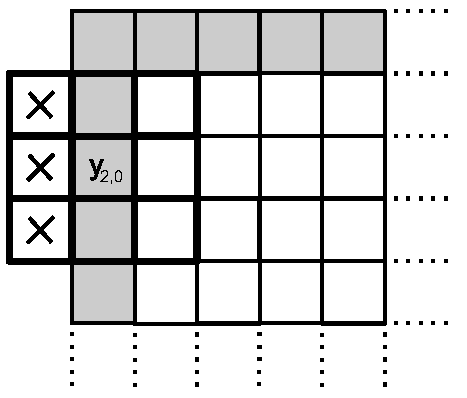
\includegraphics[scale=0.5]{figs/StencilBorder.eps}
\end{center}
\caption{Application of a 3x3 stencil in the border region}
\label{fig:StencilBorder}
\end{figure}

When implementing convolution, an immediate concern is what to do when the stencil ``falls off'' the edge of the array. For example, Figure \ref{fig:StencilBorder} shows the application of a 3x3 stencil in this circumstance. The white squares indicate the \emph{internal} region, where the stencil is entirely within the array. The grey squares indicate the \emph{border}, where part of the stencil falls outside. There are several ways of handling the border case, with two popular options being to return a constant value (like zero) for out-of-bounds elements, or to return the same value as the nearest in-bounds element. 

With the array sizes commonly encountered during image processing, only a tiny fraction of the elements are in the border region. This fact implies that for optimal performance, we should avoid testing for the border each time we compute an element. To achieve this, we represent the \emph{partitioning} of the array into various regions directly. Partitioning allows us to define the result array using element functions specialised to each region, and guarantee that the one producing the internal elements is not applied in the border region. In effect, partitioning the array allows us to lift the \textbf{if}-expression that tests for the border out of the main loop of our program, and have the library code construct the border and internal regions separately. With partitioned arrays, it does not matter if the element function for the border takes a little longer to evaluate than the one for the internal region, as the former is only applied a small number of times. Provided the simpler, internal case is well optimised, we will still get good overall performance. 


% ------------------------------------- FIG
\begin{figure}
\begin{small}
\begin{code}
data Array sh a
   = Array       { arrayExtent  :: sh
                 , arrayRegions :: [Region sh a] }
data Region sh a
   = Region      { regionRange  :: Range sh
                 , regionGen    :: Generator sh a }
data Range sh 
   = RangeAll
   | RangeRects  { rangeMatch   :: sh -> Bool
                 , rangeRects   :: [Rect sh] }
data Rect sh
   = Rect sh sh

data Generator sh a
   = GenManifest { genVector   :: Vector a }	
	
   | forall cursor. 
     GenCursored { genMake     :: sh -> cursor
                 , genShift    :: sh -> cursor -> cursor
                 , genLoad     :: cursor -> a }
\end{code}
\end{small}
\caption{New Repa array types}
\label{fig:NewRepaArrays}
\end{figure}


Our new data types are shown in Figure \ref{fig:NewRepaArrays}. An @Array@ is defined as an extent, and a list of distinct @Regions@. In the rank-2 (two-dimensional) case the extent will represent the width and height of the array. Each region has a @Range@ that defines the set of indices belonging to the region. A @Range@ can either be @RangeAll@, which indicates the entire array, or a @RangeRects@ which gives a list of rectangles (of arbitrary rank). Given a @RangeRects@, we can determine whether a particular index is inside the range either by checking whether it falls in any of the @Rects@, or using the predicate @rangeMatch@. This predicate gives the same result as the former, but can use a more efficient implementation than checking each @Rect@ individually. In general, for ``local'' array operations such as indexing a single element, we use the predicate to quickly determine which region the provided index is in. In contrast, @rangeRects@ is used when forcing the entire array, and allows us to create a loop specialised to each region. 

Each @Region@ also has a @Generator@ that encodes how the array elements in that region should be computed. As before, generators of @Manifest@ arrays are just flat vectors of unboxed values that hold the elements in row-major order. Delayed arrays are now represented in \emph{cursored} form. The cursored representation allows us to share indexing computations when forcing adjacent array elements, which is discussed further in \S\ref{sec:SharingAndCursoredArrays}. The regions of a partitioned array must provide \emph{full coverage}, meaning that every array element must be within some region. Regions are permitted to overlap, with the first one in the list taking precedence. Using overlapping allows us to define a default value for array elements with a @RangeAll@, while carving out specific areas with a @RangeRects@ earlier in the list.
 
In general, partitioning an array allows us to generate loops specialised to each region. Specialisation can occur on both a per-element and per-region basis. An example of the first is the optimisation of border handling, which we discussed earlier. An example of the second is to use different loop code to evaluate regions of different sizes. For example, when evaluating a region that is short and wide it is best to operate in a row-wise manner, computing an entire row before moving to the next. This helps to recover sharing between horizontally adjacent elements. In contrast, to evaluate a region that is tall but thin it is best to operate column-wise, to exploit sharing between vertically adjacent elements. As the @Region@ type provides a direct description of the size of each region, we can specialise the library code based on this information. The user invokes the appropriate specialisation automagically with each application of @force@. We discuss specialisation further in \S\ref{sec:FillingTheArray}.


% -----------------------------------------------------------------------------
\subsection{Bounds Checking and co-Stencils}
\label{sec:CoStencils}
Firstly, with respect to bounds checking, we sheepishly admit that the old version of Repa didn't actually do any. This issue was mentioned in \cite{Keller:repa}. As such, it was possible for buggy client programs to crash at runtime. The trouble is that bounds checking each array access adds a substantial overhead, and the comparison and branching constructs involved interfere with fusion. We tried adding it, by having the @Data.Vector@ library check each of the indexing operations on the underlying manifest array, but this resulted in a 35\% slowdown for our Laplace example applied to a 300x300 array. 

Ultimately, the problem is that client code written by the user of a library is ``untrusted'', meaning that the library must assume it will index out-of-bounds elements. With respect to the code in Figure \ref{fig:LaplaceIndex}, without a more ``heavy weight'' technology like dependent types, or some clever analysis, the compiler cannot prove that when the predicate @isBorder@ succeeds, the indexing operations in the @else@ branch of @elemFn@ are guaranteed to be valid. This problem is compounded by the fact that to support shape polymorphism we must check indices of arbitrary rank against the array bounds. Failing that we could check the linear indexing of the underlying manifest vector, but we would still need to manage the mapping between these indices and the original indices of arbitrary rank.

Our solution to this problem is to invert the relationship between the stencil definition (@elemFn@) and the source array. Instead of having the (untrusted) @elemFn@ fetch elements from the source array itself, we instead write the client code to combine source elements fed to it by the (trusted) library. This distinction is similar to the one between recursive and co-recursive functions in stream fusion \cite{Coutts:stream-fusion}, where the latter is the ``co-stencil'' case. Related work on Ypnos \cite{Orchard:ypnos} mentions the co-monadic structure of grid computations, but does not discuss the relationship with bounds checking. 

Figure \ref{fig:Stencils} gives the data type that represents stencils, while Figure \ref{fig:NewSolveLaplace} contains our new implementation of @solveLaplace@. Figure \ref{fig:Stencils} also gives the definition of @makeStencil@ which is a utility function defined by our library. The type @Stencil sh a@ specifies a stencil function of shape @sh@ that operates on arrays of element type @a@. It consists of a size such as @Z:.3:.3@ for the 3x3 case, as well as a zero value and accumulator function which define a fold operation over array elements. Figure \ref{fig:NewSolveLaplace} shows how to define the Laplace stencil. The @iterateBlockwise@ function repeatedly applies its parameter function to an array, forcing it after each iteration. In this and latter code we have elided @INLINE@ pragmas, as well as the @Shape@ and @Elt@ type class constraints to save space. We have also elided explicit matches against the input arrays @arrBoundMask@, @arrBoundValue@ and @arrInit@ that require them to be manifest. These matches are needed in our concrete implementation for performance reasons, but we hope to improve the compiler so they are not required in future. This is discussed further in \S\ref{sec:MultiStage}. 

The lambda abstraction in the definition of @laplace@ defines the \emph{coefficient function} for the Laplace stencil. The coefficient function gives the coefficients for each position in the stencil, and has type @(sh -> Maybe a)@. It gives the coefficient at a particular offset from the \emph{focus} of the stencil, or if that coefficient is zero it returns @Nothing@ instead. Handling of zeros is discussed further in the next section. As a syntactic convenience, our library also provides some Template Haskell code to make listing the coefficients easier. An example of this syntax is in the @niceLaplace@ function of  Figure \ref{fig:NewSolveLaplace}.
 
The operation of computing the sum-of-products of array elements and stencil coefficients is defined by the @Just@ case of @makeStencil@. We could have embedded the coefficient function directly in the definition of @Stencil@, but instead define stencils in terms of a more general fold operation. Using a fold leaves the door open for other stencil-like operations that are not expressed as a sum-of-products, such as the creation of a histogram of the neighbourhood of each pixel.

Returning to the issue of bounds checking, with our new definitions, client code does not need direct access to the source array at all. All of the library functions used in Figure \ref{fig:NewSolveLaplace} operate on the whole array at a time, and their safety depends on the correctness of the library, instead of the correctness of the client.

Finally, we note that in virtually all related work using imperative languages it is simply assumed that bounds checking is not performed. The focus of recent papers such as \cite{Datta:stencil-computation-autotuning} and \cite{Krishnamoorthy:auto-paralellization-of-stencils} is usually on optimising cache usage, and they presume the existence of correct, heavily optimised straight line code for computing the individual array elements. In contrast, we are trying to produce a (safe!) general purpose functional array library, which also has support for efficient stencil convolution. 

% ----------------- FIG
\begin{figure}
\begin{small}
\begin{code}
data Stencil sh a
   = Stencil { stencilSize  :: sh 
             , stencilZero  :: a
             , stencilAcc   :: sh -> a -> a -> a }

makeStencil :: sh -> (sh -> Maybe a) -> Stencil sh a
makeStencil ex getCoeff
 = Stencil ex 0 
 $ \ix val acc
    -> case getCoeff ix of
          Nothing     -> acc
          Just coeff  -> acc + val * coeff
\end{code}
\end{small}
\caption{Stencils and stencil construction}
\label{fig:Stencils}
\end{figure}


% ----------------- FIG
\begin{figure}
\begin{small}
\begin{code}
solveLaplace :: Int -> Image -> Image -> Image -> Image
solveLaplace steps arrBoundMask arrBoundValue arrInit
 = iterateBlockwise steps arrInit
 $ zipWith (+) arrBoundValue 
 . zipWith (*) arrBoundMask
 . map (/ 4) . mapStencil2 (BoundConst 0) laplace

laplace :: Stencil sh a
laplace     =  makeStencil (Z :. 3 :. 3)
            $ \ix -> case ix of
                      Z :.  0 :.  1 -> Just 1
                      Z :.  0 :. -1 -> Just 1
                      Z :.  1 :.  0 -> Just 1
                      Z :. -1 :.  0 -> Just 1
                      _             -> Nothing

niceLaplace :: Stencil sh a
niceLaplace =  [stencil2| 0 1 0
                          1 0 1 
                          0 1 0 |]
\end{code}
\end{small}	
\caption{Stencil based Laplace function}
\label{fig:NewSolveLaplace}
\end{figure}


% -----------------------------------------------------------------------------
\subsection{Zeros in Stencil Definitions}
Although the stencils we use often contain zero-valued coefficients, we want to avoid wasting cycles performing the corresponding multiplications, as they do not contribute to the final sum of products. The simple, neat and \emph{wrong} solution is to allow terms of the form $0*x$ in the intermediate code, but then add a GHC rewrite rule \cite{PeytonJones:playing-by-the-rules} to implement the obvious identities $0*x \equiv 0$ and $x+0 \equiv x$. Unfortunately, the first one of these is invalid for standard \mbox{IEEE-704} floating point numbers because the operation $0*\infty$ is supposed to produce NaN (Not a Number). Although this hardly matters for image processing, we still don't want to add the rule as it would apply globally and we risk breaking other code. Instead, we define the coefficient function to return @Nothing@ where the stencil does not apply, and use this to skip over the associated term in @makeStencil@. Nevertheless, in the literature, stencils are usually specified using zeros. Due to this we allow zeros in our Template Haskell version, but eliminate them while desugaring to the coefficient function. 



\section{Sharing and Cursored Arrays}
\label{sec:SharingAndCursoredArrays}
\label{sec:EvaluationOrder}

Suppose we apply a 3x3 stencil to a single internal point in an image, and that every coefficient is non-zero. At the least, this application would require nine floating point values to be loaded from the source array, and one store to the result. Now, as the computation of a single point in the result does not depend on any others, we can evaluate elements of the result in an arbitrary order. This makes stencil convolution an embarrassingly parallel operation, which gives us much flexibility in the implementation. 

However, as we want our convolution to run with good absolute performance on a finite number of processors, it is often better to impose a specific order of evaluation to improve efficiency. Figure \ref{fig:OverlappingSupport} shows the evaluation of four horizontally adjacent points. If we were to evaluate each of these points independently, we would need $4 \times 9 = 36$ loads of the source array, and four stores to the result. However, evaluating all four points in one operation requires only 18 loads, as well as the four stores to the result. There is also the potential to share the evaluation of array indices, and well as multiplications, depending on the form of the stencil.

The potential for sharing indexing computations can be seen in Figure \ref{fig:LaplaceIndexCore} which shows the Core IR for part of the inner loop of our Laplace example. Although this code only computes a single point in the result, note that the second argument to each application of @indexFloatArray#@ produces the offset into the array for each point in the stencil. Computation of these offsets is performed with the familiar expression @x + y * width@, where @x@ and @y@ are the coordinates of the element of interest. However, as the spacial relationship between the elements is fixed, we could instead compute the index of the focus (center) of the stencil, and then get to the others by adding +1/-1 or +width/-width. In the case where we compute four elements of the result array in a single operation, the potential savings for index computations are even greater. 

Recovering this sort of sharing is a well known problem in compiler optimisation and is the target of the Global Value Numbering (GVN) \cite{Alpern:detecting-equality-of-variables, Rosen:global-value-nubering} transformation performed by some compilers. Unfortunately, no current Haskell compiler implements this transform, so we are not home free yet. However, GHC can now compile via LLVM \cite{Terei:llvm-backend-for-ghc}, and LLVM \emph{does} implement a GVN pass. Provided we expose enough of the internal indexing computations, the LLVM compiler will do the rest for us. This brings us to cursored arrays.

% ----------------- FIG
\begin{figure}
\begin{center}
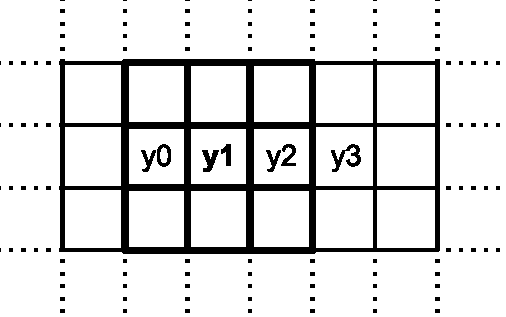
\includegraphics[scale=0.6]{figs/Stencil4.eps}
\end{center}
\caption{Overlapping support of four adjacent 3x3 stencils}
\label{fig:OverlappingSupport}
\end{figure}


% -----------------------------------------------------------------------------
\subsection{Cursored Arrays}
Recall the new Repa array representation from Figure \ref{fig:NewRepaArrays}. The definition of element generators is repeated below for reference. 

\begin{small}
\begin{code}
data Generator sh a
   = GenManifest { genVector :: Vector a }	
		
   | forall cursor. 
     GenCursored { genMake   :: sh -> cursor
                 , genShift  :: sh -> cursor -> cursor
                 , genLoad   :: cursor -> a }
\end{code}
\end{small}

A cursor is an abstract representation of an index into the array. The specific form of the cursor is defined by the \emph{producer} of the array, while the consumer must use the provided cursor functions to access elements. As hinted in the previous section, for stencil functions we represent the cursor by a linear index into the array. Given the coordinates of an element, @genMake@ computes the linear index of that element, the @genShift@ function shifts a cursor by an offset, and @genLoad@ produces the array element for a given cursor. Using cursors allows us to avoid repeated indexing computations like @x + y * width@, as we can now just compute the linear index of the centre of the stencil, then shift it around to get the other neighbouring elements.

As well as enabling sharing between index computations, cursored arrays strictly subsume our old delayed array representation. To see this, suppose we added an alternative to our @Generator@ type that implemented delayed arrays as given in \S\ref{sec:Repa}

\begin{small}
\begin{code}
  data Generator sh a
      = ...
      | GenDelayed { genGetElem  :: sh -> a }
\end{code}
\end{small}

It turns out this alternative is unnecessary, because we can write functions to convert between the delayed and cursored representations. Given a cursored array, we construct the element function for the delayed version making a cursor then immediately loading from it. Given a delayed array, we construct the cursored one by using the index itself as the cursor. This is possible due to the existential quantification of the @cursor@ type.

\begin{small}
\begin{code}
 delayedOfCursored :: Generator sh a -> Generator sh a
 delayedOfCursored (GenCursor make _ load)
         = GenDelayed (load . make)
 
 cursoredOfDelayed :: Generator sh a -> Generator sh a
 cursoredOfDelayed (GenDelayed getElem)
         = GenCursored id addIndex getElem

 addIndex :: Shape sh => sh -> sh -> sh
 addIndex = ...
\end{code}
\end{small}

To see that cursored arrays also support the delayed array approach to fusion, note that we can implement @map@ by composing its parameter with the @load@ function of the cursored array. The following code gives the definition of @mapGen@ which operates on the generator. The version for arrays is easily defined in terms of it.

\begin{small}
\begin{code}
 mapGen :: (a -> b) -> Generator sh a -> Generator sh b
 mapGen f gen
  = case arr of
     GenManifest vec  
       -> GenCursored id addDim  (\ix -> f (vec ! ix))
     GenCursored make shift load
       -> GenCursored make shift (f . load)
\end{code}
\end{small}

Finally, note that although we use cursored arrays internally to the library, there is usually no need for client programs to construct them explicitly. In the clients we have written, arrays are usually constructed with higher level utility functions, and combinators such as @map@ and @fold@ produce the same result independent of the representation of their arguments.

% -----------------------------------------------------------------------------
\subsection{Applying the Stencil}
\label{sec:ApplyingTheStencil}

% ----------------- FIG
\begin{figure}

\begin{small}
\begin{code}
data Boundary a
      = BoundConst a
      | BoundWrap
      | ...
	
mapStencil2 
  :: Boundary a -> Stencil DIM2 a
  -> Array DIM2 a -> Array DIM2 a

mapStencil2 boundary stencil@(Stencil sExtent _ _) arr
 = let (Z :. aHeight :. aWidth) = extent arr
       (Z :. sHeight :. sWidth) = sExtent

       rectsInternal    = ...
       rectsBorder      = ...
       inInternal ix    = ...
       inBorder   ix    = ...

       make  (Z:.y:.x)
        = Cursor (x + y*aWidth)
	
       shift (Z:.y:.x) (Cursor offset)
        = Cursor (offset + x + y*aWidth)

       loadBorder ix    = case boundary of ...
			
       loadInner cursor
        = unsafeAppStencil2 stencil arr shift cursor
							
   in  Array (extent arr)
        [ Region (RangeRects inBorder rectsBorder)
                 (GenCursored id addIndex loadBorder) 

        , Region (RangeRects inInternal rectsInternal)
                 (GenCursored make shift loadInner) ]


unsafeAppStencil2
  :: Stencil DIM2 a -> Array DIM2 a 
  -> (DIM2 -> Cursor -> Cursor)       -- shift cursor
  -> Cursor -> a

unsafeAppStencil2
  stencil@(Stencil sExtent sZero sAcc)
  arr@(Array aExtent [Region RangeAll (GenManifest vec)])
  shift cursor
 
  | _ :. sHeight :. sWidth  <- sExtent
  , sHeight <= 3, sWidth <= 3
  = template3x3 loadFromOffset sZero

  | otherwise = error "stencil too big for this method"

  where getData (Cursor index)
         = vec `unsafeIndex` index
		
        loadFromOffset oy ox	
         = let  offset = Z :. oy :. ox
                cur'   = shift offset cursor
           in   sAcc offset (getData cur')	


template3x3 :: (Int -> Int -> a -> a) -> a -> a
template3x3 f sZero
  =  f (-1) (-1)  $  f (-1)   0  $  f (-1)   1 
  $  f   0  (-1)  $  f   0    0  $  f   0    1   
  $  f   1  (-1)  $  f   1    0  $  f   1    1  
  $  sZero
\end{code}
\end{small}
\caption{Applying the stencil to an array}
\label{fig:MapStencil}
\end{figure}

Now that we have the definition for cursored arrays, we can see about creating one. Figure \ref{fig:MapStencil} gives the definition of @mapStencil2@ which takes the definition of a rank 2 stencil, a source array, and produces a cursored result array. The definitions of the rectangles for the border and internal regions have been elided to save space, as have the @inInternal@ and @inBorder@ predicates, though they are straightforward.

We have also elided the @INLINE@ pragmas for the @make@, @shift@ and @load@* functions. When compiling with GHC we must define these functions as separate bindings and give them @INLINE@ pragmas, instead of writing them as lambda abstractions directly in the body of the @let@ expression. Defining the functions this way ensures that when an array created with @mapStencil2@ is finally forced, these definitions are inlined into the unfolding of the @force@ function, as well as the element evaluation function @fillCursoredBlock2@ which we will discuss in the next section. If we do not do this, then the definitions would \emph{not} be appropriately inlined, and we would suffer a function call overhead for each application. We will return to this delicate point in \S\ref{sec:MultiStage}.

The values of the border elements depend on the @boundary@ parameter, and two options are shown at the top of the figure. The inner elements are defined via @unsafeAppStencil2@, which produces a function from the cursor value to the corresponding array element. Note that this function requires the provided source array to be manifest, so that elements can be extracted directly from the underling vector using @unsafeIndex@. We use @unsafeIndex@ to access the vector because this function performs no bounds checks, so we do not suffer the associated overhead. The safety of these accesses depends on the correctness of our library code, namely the @rectsInternal@ list from @mapStencil2@, so that @loadInner@ is not applied too close to the border.

Computation of the inner array elements is performed by the @loadFromOffset@ and @template3x3@ functions. The latter spells out every possible offset from the centre of a 3x3 stencil. We must spell out these offsets ``long hand'' instead of writing a recursive function to compute the result because we need each application of @f@ to be specialised for the provided offset. During compilation, @f@ will be bound to a coefficient function like the one defined in @laplace@ of Figure \ref{fig:NewSolveLaplace}. In effect, we are using @template3x3@ to select every possible coefficient that the coefficient function could have defined. By virtue of @makeStencil@ of Figure \ref{fig:Stencils}, if the coefficient function returns a valid coefficient for a particular offset then we end up with a term that multiplies that coefficient with data from the source array. If not, then the @Nothing@ branch of @makeStencil@ comes in to play and the result is unperturbed. Note that this mechanism permits us to use any stencil that \emph{fits inside} the 3x3 template. For example, stencils of size 3x1 and 2x2 also work.

Sadly, the fact that we must spell out every possible offset means that our @unsafeAppStencil2@ function is limited to handling stencils of a particular maximum size. In this case we have set the maximum to 3x3, so that it fits on the page. However, the limit is easy to increase and our concrete implementation currently uses 7x7. Limiting the size of the stencil in this way does not affect what coefficients or zero elements can be used, it just requires the entire stencil to fit inside the template. If we had instead written a recursive version of the template function, then GHC would not inline it, killing performance. In general, repeatedly inlining a recursive function may not terminate, leading to divergence at compile time. We can think of several ways of addressing this issue, but all require modification to the compiler, and we defer further discussion to \S\ref{sec:ManualUnwinding}. If the stencil does not fit inside the template then we fall back to the standard approach of loading the coefficients into a manifest array and iterating directly over that. This gets the job done, but obviously misses out on the benefits of the cursored approach. A follow on effect of spelling out every offset is that it also limits @mapStencil2@ to arrays of rank 2. It is straightforward to write versions for other ranks, as the general structure is the same as the rank-2 case, but we don't have a way of doing this polymorphically.

Finally, note that @unsafeAppStencil2@ defines a function between a cursor and a single array element. The task of actually filling the result array while exposing sharing between adjacent elements is performed by @fillCursoredBlock2@, which we discuss in the next section.


% -----------------------------------------------------------------------------
\subsection{Filling the Array, and Interaction with LLVM}
\label{sec:FillingTheArray}

% ----------------- FIG
\begin{figure}
\begin{small}
\begin{code}
case quotInt# ixLinear width  of { iX ->
case remInt#  ixLinear width  of { iY -> 
case +# iX (*# iY width) of { ixCenter ->
 writeFloatArray# world arrDest ixLinear
  (+##  (indexFloatArray# arrBV 
          (+# arrBV_start (+# (*# arrBV_width iY) iX)))
   (*## (indexFloatArray# arrBM 
          (+# arrBM_mask  (+# (*# arrBM_width iY) iX)))
    (/## (+## (+## (+##
      (indexFloatArray# arrSrc 
       (+# arrSrc_start (+# ixCenter width)))
      (indexFloatArray# arrSrc
       (+# arrSrc_start (+# ixCenter 1))))
      (indexFloatArray# arrSrc
       (+# arrSrc_start (+# ixCenter (-1)))))
      (indexFloatArray# arrSrc
       (+# arrSrc_start (+# ixCenter (*# (-1) width)))))
     4.0))) }}
\end{code}
\end{small}
\caption{New core IR for Laplace with index sharing}
\label{fig:NewLaplaceIndexCore}
\end{figure}


% ----------------- FIG
\begin{figure}
\begin{small}
\begin{code}
fillCursoredBlock2
 :: IOVector a                   -- vector to write into
 -> (DIM2   -> cursor)           -- makeCursor
 -> (DIM2   -> cursor -> cursor) -- shiftCursor
 -> (cursor -> a) -> Int         -- loadElem, width
 -> Int -> Int -> Int -> Int     -- coords of block
 -> IO ()
fillCursoredBlock2 !vec !make !shift !load
   !width !x0 !y0 !x1 !y1 = ... fillRow4 ...
 where 
    fillRow4 !y !x    -- fill a single row in the block
     | x + 4 > x1     = ... -- less than 4 elems remaining
     | otherwise
     = do let srcCur0 = make  (Z:.y:.x)
          let srcCur1 = shift (Z:.0:.1) srcCur0
          let srcCur2 = shift (Z:.0:.1) srcCur1
          let srcCur3 = shift (Z:.0:.1) srcCur2

          let val0    = load srcCur0
          let val1    = load srcCur1
          let val2    = load srcCur2
          let val3    = load srcCur3
          touch val0; touch val1; touch val2; touch val3

          let !dstCur0 = x + y * width
          unsafeWrite vec (dstCur0)     val0
          unsafeWrite vec (dstCur0 + 1) val1
          unsafeWrite vec (dstCur0 + 2) val2
          unsafeWrite vec (dstCur0 + 3) val3
          fillRow4 y (x + 4)
\end{code}	
\end{small}
\caption{Block evaluation function for cursored DIM2 arrays}
\label{fig:BlockEvaluation}
\end{figure}

Using our original @force@ function (not shown), but with cursored arrays, produces a loop whose inner fragment consists of the Core IR shown in Figure \ref{fig:NewLaplaceIndexCore}. The loop as a whole iterates through the linear indices of the result vector. In the body, each linear index (@ixLinear@) is converted to a rank-2 index, then back to a cursor value @ixCenter@. As the source and destination arrays have the same dimensions, @ixLinear@ and @ixCenter@ will have the same value. The intermediate conversion is successfully eliminated by the LLVM optimiser, so doesn't appear in the object code. 

Note how each of the elements of the source array are indexed relative to the cursor @ixCenter@. To recover sharing between adjacent elements we must evaluate several in the same iteration, which requires a new version of @force@. The inner loop of this new version is defined by @fillCursoredBlock2@ in Figure \ref{fig:BlockEvaluation}, which is also part of the library. This function takes a mutable @IOVector@, along with the functions that form a cursored array, and uses them to fill a rectangular block in the vector. Parallelism is introduced by having @force@ fork off several threads, with each filling a different block of array elements. Performing block-wise evaluation also improves cache usage, as the evaluation of each successive row in a block usually requires source elements that were loaded into cache during the evaluation of previous rows.

In the definition of @fillCursoredBlock2@ we have manually applied the \mbox{\emph{unroll-and-jam}} transformation \cite{Carr:unroll-and-jam} to evaluate groups of four consecutive elements per iteration. We operate row-wise, which is good for regions that are at least four elements wide. To evaluate narrow regions such as the one pixel wide left-hand border from Figure \ref{fig:StencilBorder} it is better to operate column-wise, using a separate filling function derived from the presented code.

The @touch@ function in the inner loop is used to place a dependency on the computed array values, and prevent GHC from floating the @srcCur@* and @val@* bindings into the applications of @unsafeWrite@. The @touch@ function has the following type, and is defined in terms of the GHC primitive operation @touch#@. 

\begin{small}
\begin{code}
  touch :: Elt a => a -> IO ()
\end{code}
\end{small}

We need all four element values to be computed \emph{before} any of them are written to the result array. This is to avoid a hairy interaction with the LLVM optimiser. Specifically, LLVM does not know that the low-level representation of the source and result arrays do not alias, nor does it know that the result array and GHC \emph{stack} do not alias. Any write to the result array or stack is assumed to also modify the source array, which invalidates data held in registers at that point. This in turn breaks the GVN (Global Value Numbering) optimisation which we depend on to recover sharing.

The disassembled x86\_64 object code for the inner part of our loop is given in Figure \ref{fig:SobelAssembly}. This is for the $Sobel_X$ stencil shown in Figure \ref{Fig:ExampleKernels}. Floating point loads are marked with round bullets, while floating point stores are marked with diamonds. There are 18 loads and 4 stores, and examining Figure \ref{fig:OverlappingSupport} shows that this is the optimal number for such a 3x3 stencil. However, we still have a slight inefficiency due to aliasing issues. Note the repeated instruction @mov 0x6(rbx),rcx@ after each floating point store. The @rbx@ register contains a pointer to the stack, and each floating point store invalidates the previously loaded value in @rcx@. Aliasing becomes more of a problem when compiling to architectures with insufficient floating point registers. For example 32bit x86 code can only address 8 of the 16 XMM registers available in 64bit mode. If the LLVM compiler runs out of registers then it spills values to the stack, which also invalidates previously loaded values. Fixing this will require more work on GHC's LLVM backend, and/or a type system or analysis that recovers the non-aliasing of heap objects.

Finally, note that the optimal number of elements to compute per iteration depends on the form of the stencil, namely how many coefficients overlap when several stencils are placed side-by-side. Computing too few elements per iteration limits how much sharing can be recovered, while computing too many increases register pressure and can cause intermediate values to be spilled to the stack. Currently, we always compute four at once, which works well for most 3x3 stencils. In future work we intend to add a size-hint to our @Array@ type, which would be set by @mapStencil2@. The @fillCursoredBlock2@ function would use this hint to choose between several loops, all with the same form as @fillRow4@, but computing a different number of elements per iteration.


% ------------------------------------- FIG

% Macros for formatting assembly code.
\newcommand{\asm}[3]	
{		& \hspace{-2em} {\tt #1:} 
		& \hspace{-2em} {\tt #2} 
		& \hspace{-1em} {\tt #3} \\}

\newcommand{\aasm}[4]
{\hspace{-1em} #1 \hspace{-3em}  
		& \hspace{-2em} {\tt #2:}
		& \hspace{-2em} {\tt #3}
		& \hspace{-1em} {\tt #4} \\}

\newcommand{\lasm}[3]	{ \aasm{$\bullet$}	{#1}{#2}{#3} }
\newcommand{\sasm}[3]	{ \aasm{$\diamond$}	{#1}{#2}{#3} }


\begin{figure}
\begin{minipage}[b]{0.5\linewidth}
\begin{tiny}
\begin{tabular}{lrll}
\asm	{9b0}	{mov}	{0x2e(rbx), rcx}
\asm	{9b4}	{mov}	{0x1e(rbx), rdx}
\asm	{9b8}	{mov}	{rdx, rsi}
\asm	{9bb}	{imul}	{rcx, rsi}
\asm	{9bf}	{mov}   {0x36(rbx), rdi}
\asm	{9c3}	{lea}   {0x4(r14,rdi,1), r8}
\asm	{9c8}	{add}   {r14, rdi}
\asm	{9cb}	{lea}   {0x1(rcx), r9}
\asm	{9cf}	{imul}  {rdx, r9}
\asm	{9d3}	{lea}   {0x2(r9,rdi,1), r10}
\asm	{9d8}	{mov}   {0x6(rbx), r11}
\asm	{9dc}	{mov}   {0xe(rbx), r15}
\\
\lasm 	{9e0}	{movss} {0x10(r15,r10,4), xmm7}
\asm	{9e7}	{lea}   {(r8,r9,1), r10}
\lasm	{9eb}	{movss} {0x10(r15,r10,4), xmm8}
\asm	{9f2}	{subss} {xmm7, xmm8}
\asm	{9f7}	{lea}   {(r8,rsi,1), r10}
\lasm	{9fb}	{movss} {0x10(r15,r10,4), xmm9}
\asm	{a02}	{addss} {xmm9, xmm9}
\asm	{a07}	{addss} {xmm8, xmm9}
\asm	{a0c}	{lea}   {0x2(rsi,rdi,1), r10}
\lasm	{a11}	{movss} {0x10(r15,r10,4), xmm8}
\asm	{a18}	{movaps}{xmm8, xmm10}
\asm	{a1c}	{mulss} {xmm0, xmm10}
\asm	{a21}	{addss} {xmm9, xmm10}
\asm	{a26}	{dec}   {rcx}
\asm	{a29}	{imul}  {rdx,rcx}
\asm	{a2d}	{add}   {rcx,r8}
\\
\lasm	{a30}	{addss} {0x10(r15,r8,4), xmm10}
\asm	{a37}	{lea}   {0x1(r9,rdi,1), rdx}
\lasm	{a3c}	{movss} {0x10(r15,rdx,4), xmm9}
\asm	{a43}	{lea}   {0x3(r9,rdi,1), rdx}
\lasm	{a48}	{movss} {0x10(r15,rdx,4), xmm11}
\asm	{a4f}	{subss} {xmm9, xmm11}
\asm	{a54}	{lea}   {0x3(rsi,rdi,1), rdx}
\lasm	{a59}	{movss} {0x10(r15,rdx,4), xmm12}
\asm	{a60}	{addss} {xmm12, xmm12}
\asm	{a65}	{addss} {xmm11, xmm12}
\asm	{a6a}	{lea}   {0x1(rsi,rdi,1), rdx}
\lasm	{a6f}	{movss} {0x10(r15,rdx,4), xmm11}
\asm	{a76}	{movaps}{xmm11, xmm13}
\asm	{a7a}	{mulss} {xmm0, xmm13}
\asm	{a7f}	{addss} {xmm12, xmm13}
\asm	{a84}	{lea}   {0x3(rcx,rdi,1), rdx}
\lasm	{a89}	{addss} {0x10(r15,rdx,4), xmm13}
\\
\end{tabular}
\end{tiny}
\end{minipage}
% --------------------
\begin{minipage}[b]{0.5\linewidth}
\begin{tiny}
\begin{tabular}{lrll}
\asm	{a90}	{lea}	{(rdi,r9,1), rdx}
\lasm	{a94}	{subss}	{0x10(r15,rdx,4), xmm7}
\asm	{a9b}	{addss}	{xmm8, xmm8}
\asm	{aa0}	{addss}	{xmm7, xmm8}
\asm	{aa5}	{lea}	{0x1(rcx,rdi,1), rdx}
\asm	{aaa}	{lea}	{0x2(rcx,rdi,1), r8}
\asm	{aaf}	{lea}	{(rdi,rsi,1), r10}
\lasm	{ab3}	{movss}	{0x10(r15,r10,4), xmm7}
\asm	{aba}	{mulss}	{xmm0, xmm7}
\asm	{abe}	{addss}	{xmm8, xmm7}
\lasm	{ac3}	{movss}	{0x10(r15,r8,4), xmm8}
\asm	{aca}	{addss}	{xmm8, xmm7}
\asm	{acf}	{lea}	{(rdi,rcx,1), r8}
\lasm	{ad3}	{subss}	{0x10(r15,r8,4), xmm7}
\\
\asm	{ada}	{add}   {rax, rdi}
\asm	{add}	{add}   {rdi, r9}
\lasm	{ae0}	{subss} {0x10(r15,r9,4), xmm9}
\asm	{ae7}	{addss} {xmm11, xmm11}
\asm	{aec}	{addss} {xmm9, xmm11}
\asm	{af1}	{lea}   {(rdi,rsi,1), r8}
\lasm	{af5}	{movss} {0x10(r15,r8,4), xmm9}
\asm	{afc}	{mulss} {xmm0, xmm9}
\asm	{b01}	{addss} {xmm11, xmm9}
\lasm	{b06}	{movss} {0x10(r15,rdx,4), xmm11}
\asm	{b0d}	{addss} {xmm11, xmm9}
\asm	{b12}	{add}   {rcx, rdi}
\lasm	{b15}	{subss} {0x10(r15,rdi,4), xmm9}
\\
\asm	{b1c}	{add}   {r14,rsi}
\sasm	{b1f}	{movss} {xmm9,0x10(r11,rsi,4)}
\asm	{b26}	{mov}   {0x6(rbx),rcx}
\sasm	{b2a}	{movss} {xmm7,0x14(rcx,rsi,4)}
\asm	{b30}	{subss} {xmm11,xmm13}
\asm	{b35}	{mov}   {0x6(rbx),rcx}
\sasm	{b39}	{movss} {xmm13,0x18(rcx,rsi,4)}
\asm	{b40}	{subss} {xmm8,xmm10}
\asm	{b45}	{mov}   {0x6(rbx),rcx}
\sasm	{b49}	{movss} {xmm10,0x1c(rcx,rsi,4)}
\asm	{b50}	{lea}   {0x8(r14),rcx}
\asm	{b54}	{lea}   {0x4(r14),r14}
\asm	{b58}	{cmp}   {0x26(rbx),rcx}
\asm	{b5c}	{jle}   {9b0}
\end{tabular}
\end{tiny}
\end{minipage}

\caption
	{ x86\_64 assembly for $Sobel_X$  applied to four consecutive pixels. 
	  FP loads and stores are marked with $\bullet$ and $\diamond$. }
\label{fig:SobelAssembly}
\end{figure}




%!TEX root = ../Main.tex


% -----------------------------------------------------------------------------
\begin{figure*}[t]
\begin{center}
\begin{tabular}{lccccrccc}
Benchmark 
        & Input size 
        & Stream (ms) 
        & \multicolumn{2}{c}{Flow (ms)} 
        & \multicolumn{2}{c}{Unfused Flow (ms)}  
        & \multicolumn{2}{c}{Hand-fused C (ms)}    \\
\hline
Dot Product &  $10^8$    & 655    & 489    &  (75\%) & 1,096  & (167\%)  & 474      & (72\%) \\
MapMap      &  $10^8$    & 842    & 636    &  (75\%) & 842    & (100\%)  & 615      & (73\%) \\
FilterSum   &  $10^8$    & 505    & 430    &  (85\%) & 1,132  & (224\%)  & 344      & (68\%) \\
FilterMax   &  $10^8$    & 567    & 521    &  (91\%) & 1,496  & (263\%)  & 360      & (63\%) \\
NestedFilter&  $10^8$    & 485    & 420    &  (86\%) & 1,202  & (247\%)  & 376      & (77\%) \\
QuickHull   &  $10^7$    & 419    & 208    &  (49\%) & 857    & (204\%)  & 183      & (43\%) \\
\end{tabular}
\caption{Benchmark Results for Flow Fusion}
\label{f:benchmark-table}
\end{center}
\end{figure*}


% -----------------------------------------------------------------------------
\section{Benchmarks}
\label{s:Benchmarks}
Benchmarks were conducted on a MacBook Pro with 2.8GHz Intel Core i7 with 8GB of RAM. Source code is available from the @repa-plugin@ darcs repository. 

We use micro-benchmarks because our fusion system addresses these specific programming patterns, rather than being an improvement on the ambient performance of the program --- as with optimizations like pointer tagging~\cite{Marlow:pointer-tagging}.

For each benchmark we compare four implementations:
\begin{itemize}
\item \emph{Stream}: using stream fusion~\cite{Coutts:stream-fusion} and unboxed vectors;\footnote{from the @vector@ library on Hackage}

\item \emph{Flow}: using our new Flow fusion framework;

\item \emph{Unfused Flow}: using our Flow API but without the plugin;

\item \emph{Hand-fused}: hand written and fused C code.
\end{itemize}

The Unfused Flow versions use the exact same code as the Flow versions, except they are compiled without the plugin that actually performs the fusion transformation. In this case the benchmarks are compiled via a fallback implementation of the user-facing API of Figure~\ref{f:SeriesOperators}, implemented in terms of standard stream fusion~\cite{Coutts:stream-fusion}. The fallback implementation provides a quick compilation path for people that do not want to install the plugin or care about the last ounce of 
performance, as well as a convenient way of testing the plugin itself.


% -----------------------------------------------------------------------------
\subsection{Dot Product}
A pair of two-dimensional vectors are multiplied element-wise and the results summed. Each two dimensional vector is stored as two arrays of integers, giving four arrays in total. As discussed in \S\ref{s:streams-zipWith}, code compiled with stream fusion produces a loop counter for each vector. With flow fusion the concretization phase (\S\ref{s:Concretization}) naturally causes loop counters to be shared. This provides a 25\% speedup over stream fusion and puts us on par with the reference C implementation. 


% -----------------------------------------------------------------------------
\subsection{MapMap}
The elements of a vector of integers are doubled, and the resulting vector has a constant added in one operation and subtracted in another. With stream fusion the first result is materialized in memory, and then read back by each of the subsequent vector operations. With flow fusion the first result is not materialized, which also puts us on par with the reference C implementation.


% -----------------------------------------------------------------------------
\subsection{FilterSum}
A vector of integers is filtered and the elements of the original and result vectors are separately summed. The result vector and both sums are returned in a 3-tuple. With stream fusion the code uses three separate loops, one for each operator. With flow fusion the code uses a single loop that sums both the original and result vectors while constructing the result. 

Although the Core code produced by flow fusion is optimal, the low-level object code suffers from pointer aliasing problems. The back-end code generator does not know that the input vector does not alias with the result vector, nor that writes to the element data of the result do not affect its starting offset field. Ultimately, the length field of the first vector, and starting offsets for both vectors are repeatedly read in the inner loop. The C compiler can infer correct aliasing information, and thus saves three memory reads per loop iteration.


% -----------------------------------------------------------------------------
\subsection{FilterMax}
This is the @filterMax@ example described earlier. With stream fusion the filtered result vector must be read back from memory to sum its elements. With flow fusion the sum is performed in the same loop as the filter. Similarly to the FilterSum benchmark, although the Core code is optimal, low level pointer aliasing problems in the object code prevent us from matching the performance of the C version.


% -----------------------------------------------------------------------------
\subsection{NestedFilter}
An input vector is filtered, this result filtered again by another predicate, and both results are returned in a tuple. With stream fusion the first result is constructed in memory and then read back to perform the second filter. With flow fusion both results are constructed in the same loop and the first is not read back. As mentioned in \S\ref{s:SchedulingPacks} this benchmark uses two nested applications of @mkSel@, thus the Core code contains two nested guards. 


% -----------------------------------------------------------------------------
\subsection{QuickHull}
QuickHull finds the smallest convex hull of a set of points in the 2-d plane. The algorithm operates in two phases. The first is an initialization phase where we determine the left-most and right-most points in the input set. If these results are computed in two separate fold operations then stream fusion cannot fuse this code. In the second phase, we need to determine the set of points above a cutting line and also the point furthest from it. This is a @filterMax@-like operation that stream fusion can also not fuse.




\section{Challenges of Array Fusion}
In this section we summarise the main challenges we have encountered with this work, and suggest avenues for future research.


% -----------------------------------------------------------------------------
\subsection{Lack of Support for SIMD Operations}
At face value, using 4-way SIMD instructions such as available in the SSE or MMX set has the potential to improve the performance of certain algorithms 4-fold. This assumes that our application isn't memory bound, though note that even a 1024x1024 image of 32bit floats sits comfortably in the 12MB cache of our test machine. Of course, the fact we are using a super-scalar architecture implies that we won't necessarily get a 4-fold speedup on a linear instruction stream, though we note that using SIMD also effectively increases the size of the register set. Expanding the register set would help to avoid the aliasing issues discussed in \S\ref{sec:SharingAndCursoredArrays}. Whether it's better to introduce SIMD instructions in Haskell code, or have the LLVM compiler reconstruct them is an open question. 


% -----------------------------------------------------------------------------
\subsection{Manual Unwinding of Recursive Functions}
\label{sec:ManualUnwinding}
As mentioned in \S\ref{sec:ApplyingTheStencil} we must manually unfold loops over regions and rectangles as GHC avoids inlining the definitions of recursive functions. The nice way to fix this would be some form of supercompilation \cite{Bolingbroke:supercompilation, Mitchell:supercompilation}. Support for supercompilation in GHC is currently being developed, though still in an early stage. Failing that, we could perhaps add a new form of the @INLINE@ pragma that unfolded recursive functions indiscriminately, or a fixed number of times. The downside of the first is potential divergence at compile time, the downside of the second is lack of generality.


% -----------------------------------------------------------------------------
\subsection{Unboxing Outside of Loops}
\label{sec:UnboxingOutsideOfLoops}
As mentioned in \S\ref{sec:CoStencils} we currently need to add some boilerplate code to functions such as @solveLaplace@ to ensure that arrays are unboxed outside of loops, instead of once per iteration. This code has the following form, and is applied to each input array:

\begin{small}
\begin{code}
  f arr@(Array _ [RangeAll (GenManifest _)]) 
   = arr `deepSeqArray` ...
\end{code}
\end{small}

The @deepSeqArray@ function places a demand on every boxed object in @arr@ before returning its second argument. The pattern match is added to functions that we know will only ever be passed forced arrays, and ensures that indexing operations in the body of the function are specialised for this case. The root problem is that unboxing operations are represented as case matches, but while let-bindings can be floated out of loops, case matches cannot. We hope to fix this particular infelicity in the near future.


% -----------------------------------------------------------------------------
\subsection{\texttt{INLINE}s and Whole Program Compilation}
\label{sec:MultiStage}

As almost every function definition in the Repa library has an @INLINE@ pragma, we are essentially doing whole program computation, at least for the array part. In a syntactic sense, the @INLINEs@ do clutter up the code, and we have spent hours hunting performance problems that were due to a lack of an @INLINE@. In a deeper sense, we feel uneasy about the fact that performance depends so heavily on the syntactic structure of the code, but we don't have a general solution for this. In \S\ref{sec:ApplyingTheStencil} we mentioned the need to write the @make@, @shift@ and @load@ functions as separate function bindings, and attach @INLINE@ pragmas. The need to write separate bindings is simply driven by the need to add @INLINE@s, as in GHC this information is attached to the name of the function binding to be inlined.

Although we could imagine adding a desugaring pass that converted the source code to the desired form, in practice we also want to manually attach inlining stage numbers to many of the bindings. Stage numbers are used to ensure that some bindings are inlined and specialised before others. This can avoid the need for the compiler to optimise large swathes of code only to discard it due to case specialisation later in the compilation.



% -----------------------------------------------------------------------------
\subsection{Promises of Purity}
\begin{figure}
\begin{small}
\begin{code}
force :: Array sh a -> Array sh a
force arr
 = unsafePerformIO
 $ do (sh, vec) <- forceIO arr
       return $ sh `seq` vec `seq` 
         Array sh [Region RangeAll (GenManifest vec)]

 where forceIO arr'
        = case arr' of
           Array sh [Region RangeAll (GenManifest vec)]
            -> return (sh, vec)
           Array sh regions
            -> do mvec <- new (size sh)
                  mapM_ (fillRegionP mvec sh) regions
                  vec  <- unsafeFreeze mvec
                  return (sh, vec)
\end{code}
\end{small}
\caption{The interface between pure and monadic code}
\label{fig:TheForce}
\end{figure}


Figure \ref{fig:TheForce} shows the code for the @force@ function that produces a manifest array from a delayed one. This function also has the distinction of being the interface between the IO code that fills the array using concurrent threads, and our pure Repa API. Constructing the pure interface consists of two aspects, which are embodied by the following functions:
\par
\begin{small}
\begin{code}
 unsafePerformIO :: IO a -> a
 unsafeFreeze    :: MVector IO a -> IO (Vector a)
\end{code}
\end{small}
\par
The @unsafePerformIO@ function breaks the monadic encapsulation of an IO action. Remembering that we're using a lazy language, this is effectively a promise by the programmer that the result can be evaluated at any time without affecting its final value. Similarly, @unsafeFreeze@ coerces a mutable vector (@MVector@) to an immutable one (@Vector@), and serves as a promise that after that point in time, the underlying data will not be mutated further. Importantly, failing to respect the two promises results in undefined behaviour at runtime, and neither of the promises can be statically checked by the compiler. Due to this, we would prefer if such promises were enforced by someone else. Actually, the @Data.Vector@ library \emph{almost} provides what we want:
\par
\begin{small}
\begin{code}
create :: (forall s. ST s (MVector (ST s) a)) -> Vector a
\end{code}
\end{small}
\par
This function takes an @ST@ action that produces a mutable vector, evaluates it, then coerces the result to an immutable one. The soundness of the coercion is guaranteed by the @ST@ state variable (@s@), which ensures that no references to the mutable vector can escape from the scope of the action that produced it \cite{Launchbury:state-threads}. Unfortunately, there is no equivalent version of @create@ for the @IO@ monad, and we need @IO@ because the primitive functions we use to implement parallelism produce @IO@ actions. 

More specifically, the @readMVar@ and @putMVar@ functions operate on mutex variables, and the result of the first can depend on the order in which concurrent threads are scheduled. Note that it is concurrency, not destructive update that is the essential problem here, as destructive update by itself can be safely encapsulated in @ST@. In related work, the type system of Deterministic Parallel Java (DPJ) \cite{adve:type-system-dpj} can express that concurrent writes to non-overlapping partitions of an array do not interfere. However, the published version of DPJ does not support parametric polymorphism of value or effect expressions. This lack of polymorphism makes it impractical to work with the higher order functions we use in Repa. Until a more fine-grained control over effects makes it into a higher-order system, it seems that we are forced to use primitives like @unsafePerformIO@ and subvert the guarantees of our purely functional language. 

On a happy note, although we can't statically check the soundness of our purifying coercions, at least they are confined to a single place in the code -- the @force@ function. This function is also the logical place for such coercions, as it converts the ``abstract'' delayed array into a concrete, manifest one.

\section{Related Work}
Approaches to the implementation of irregular parallelism roughly fall into two categories: thread-based implementations, like Manticore \cite{Fluet:2008:Manticore} or Ct \cite{ghuloum-etal:Ct}, and those based on flattening. Both have their advantages and drawbacks. With the former approach, scheduling, synchronisation, and granularity control are a concern, as well as a more restricted set of target architectures, though they do not suffer from the complexity problem described in this paper. However, the problem we describe is a fundamental issue for all flattening based approaches, and has been identified and discussed in several publications. 

The original first-order flattening transform and array representation shown in Figure~\ref{figure:OldArrayRepresentation} was introduced by Blelloch and Sabot in in \cite{Blelloch:compiling-collection-oriented-languages}. In this work the @replicate@ function is called @distribute@ when applied to scalars and @distribute-segment@ when applied to arrays. As a possible extension to the handling of conditionals they suggest operating on sparse segments instead of first eliminating gaps between them with the @pack@ operation. This idea is not elaborated further. The single example program they present (Quicksort) only uses @distribute@ and @pack@ on arrays of scalars, and thus does not suffer problems with asymptotic complexity. 

In \cite{Blelloch:vector-models} Blelloch proves that a subset of programs written with the scan-vector instruction set can be vectorised while preserving their asymptotic work and step complexity. Such programs must be both \emph{contained}, and not use indirect memory access, which is equivalent to disallowing functions to have free variables. Appendix C of the NESL manual \cite{Blelloch:nesl-3_1} gives the work complexity of vectorised programs, and states that the contents of free variables is copied across each iteration of the @apply-to-each@ (@map@) construct. Finally, in \cite{Blelloch:provable-type-and-space-efficient} the authors present a provably time and space efficient version of NESL, but the operational semantics is based around fine grained threads instead of SIMD style vectors. 

In \cite{Palmer:work-efficient-nested-data-parallelism}, Palmer et al.\ address the issue by disallowing partial applications and removing some of the problematic cases
using rewrite rules. For Haskell, ruling out partial applications to appear anywhere in a parallel context would be neither  desirable nor statically enforceable. The rewrite rules used do not fire if the offending index space transform is applied indirectly as part of another function. This is a general drawback of using rewrite rules, which can be acceptable if the rewriting only leads to a constant improvement, but not in our case, where the failure to identify problematic expressions results in asymptotically worse performance.

In \cite{Riely:flattening-improvement}, Riely and Prins solve this problem by using vectors of references, but at the time the article was written, there was no implementation, so they could not provide any experimental data as to the absolute performance. To the best of our knowledge, they have not published any further results on this approach. The suggested representation is similar to one of the states our representation can take on, for example, as a result of creating a nested vector by
collecting a number of different flat arrays in a nested one. However, the use of purely pointer based representations can lead to poor locality and complicates distribution and load balancing. It also increases garbage collection overhead, as every subarray must be traversed individually. In contrast, our approach aims at keeping the data representation as flat as possible, and only resorts to the partially flattened representation whenever the completely flat representation would lead to 
worse work complexity. 

\eject


% -----------------------------------------------------------------------------
\paragraph{Acknowledgements}
Thanks to Rami Mukhtar and Ben Lever for writing the original Canny Edge Detection code, Roman Leshchinskiy for suggesting the use of cursored arrays, and Simon Peyton Jones for describing the behaviour of the GHC simplifier.
This work was supported in part by the Australian Research Council under grant number LP0989507.

\bibliographystyle{abbrvnat}
\bibliography{Main}

\end{document}

